\documentclass[12pt,oneside,final]{siuethesis}
\usepackage{microtype} % (optional) for more beautiful typesetting
\usepackage{graphicx} 
\usepackage{hyperref} %makes links clickable
\hypersetup{colorlinks,citecolor=black,filecolor=black,linkcolor=blue,urlcolor=black} %good for electronic copy
\hypersetup{colorlinks,citecolor=black,filecolor=black,linkcolor=black,urlcolor=black}%required for paper graduate school copy
%\usepackage[alphabetic]{amsrefs} %required if using amsrefs, comment out if using bibtex
\usepackage{fixltx2e}
\usepackage{amsmath}
\usepackage{epsf}
%\usepackage{float}
\usepackage{caption}
\usepackage{subfig}
%\usepackage{subcaption}
\usepackage{listings}
\usepackage{rotating}
\usepackage{tabularx}

\usepackage{multirow}

%% controls numbering of theorems
%% this can be configured to your advisor's taste
\newtheorem{theorem}{Theorem}[chapter] %theorem number resets each chapter
\newtheorem{conclusion}[theorem]{Conclusion}
\newtheorem{condition}[theorem]{Condition}
%% conjectures, corollary, defn, etc. numbered sequentially from beginning of chapters
\newtheorem{conjecture}[theorem]{Conjecture} 
\newtheorem{corollary}[theorem]{Corollary}
\newtheorem{example}[theorem]{Example} 
\newtheorem{lemma}[theorem]{Lemma}
\newtheorem{proposition}[theorem]{Proposition}
\newtheorem{solution}[theorem]{Solution}
\theoremstyle{definition}
\newtheorem{definition}[theorem]{Definition}


\author{Bryan Orabutt}
\title{Todo: Title}

%%\advisor{John Q.\ Faculty} %% or 
\advisor{Dr.}{George L. Engel}
\secondreader{Dr.}{Bradley Noble} %% or \secondreader{Dr.}{Karl Gauss}
\thirdreader{Dr.}{Timothy York}
%\fourthreader{Karl Gauss, Sr.}
%\fifthreader{Karl Gauss, Sr.}
%\secondadvisor{Karl Gauss} %if you haves two advisors (rare) then use this line also and pass the option `twoadvisors' to the class
%\abstracttext{Chairperson: The Honorable Jill Smith} %optional -- you can use this to override the text on the abstract page; the grad school default is built-in
\submitdate{April, 2017} %date the month/year submitted to grad school, use a comma between
\copyrightyear{2017} %optional, but required if copyrighted

%% all of these are optional; defaults are shown
\major{Electrical Engineering} 
\degree{Master of Science} %can be used to specify M.A., etc.
\highestdegree{Bachelor of Science} %used if the author already has another graduate degree
\department{Electrical and Computer Engineering} 
%\departmentname{Department}
%\refname{REFERENCES} 

%\captionsetup{width=0.7\textwidth}

\begin{document}
\maketitle 

\frontmatter %signals single spacing/roman numeral pagination

\copyrightpage %optional

%%% abstracts are optional
\begin{abstract}

Todo: Abstract

\end{abstract}

\begin{acknowledgements}


Todo: acknowledgements

\end{acknowledgements}

\tableofcontents

\cleardoublepage %cause correct numbering of list of figures

\listoffigures %print list of figures page

\cleardoublepage

\listoftables

\mainmatter %signals single spacing/arabic numeral paginations


\chapter{INTRODUCTION}  %% chapter titles must be typed in all caps to conform with regulations


\section{This is a section}

Todo: introduction + sections

Figure reference example: Figure~\ref{fig:FaberRobot}

\begin{figure}[htbp!]
\centering
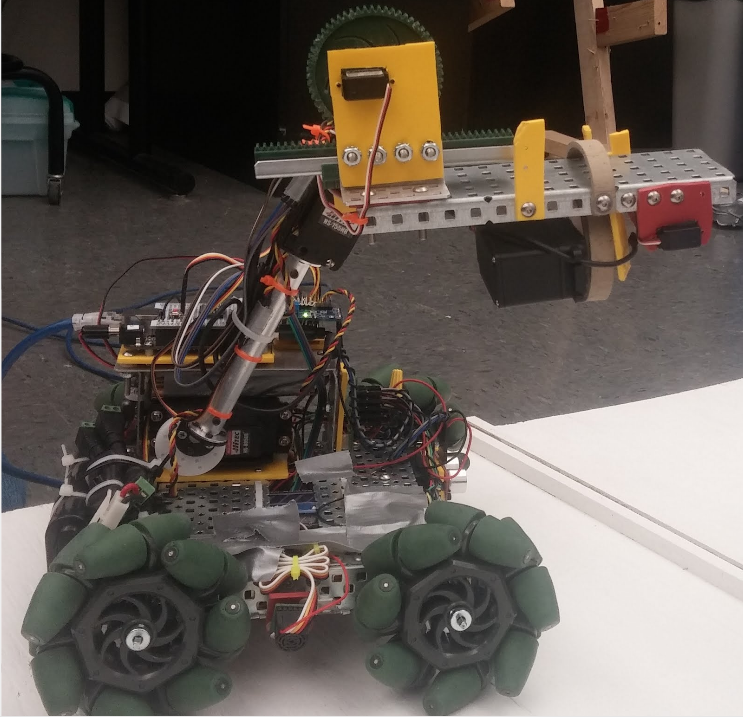
\includegraphics[scale=.6,keepaspectratio=true]{./images/FaberRobot.png} 
\caption{Authors's Robot for IEEE Competition}
\label{fig:FaberRobot}
\end{figure}

Bulleted list example:

\begin{itemize}
\item 
mechanical components to construct a mechanically-sound robot,
\item
a high-performance, small form factor computer platform that can be used for high-level decision making,
\item
an intelligent, flexible, dedicated motor controller highly integrated with the high-level compute platform, 
\item
a method to quickly and easily integrate peripheral devices into the robotic system, and
\item
a quick and convenient way to change system parameters, thus promoting experimentation.
\end{itemize}

\noindent
Numbered list example: 
\begin{enumerate}
\item
Identify a maker of mechanical robot parts which are inexpensive, easy-to-use, and flexible. Students should \textbf{not} have to machine their own parts nor should they be constrained to use a prescribed robotics kit.
\item
Identify a SBC that would be able to handle the requirements of both movement and higher level decision making.
\item
Create a custom motor controller board capable of handling all motor types which could be highly integrated with the processor tasked with higher level decision making. The board should also contain key peripherals and the ability for the user to quickly and easily add additional peripherals.
\item
Create a graphical user interface (GUI) that would allow students to quickly configure the key parameters of the robotic system.
\end{enumerate}

Table example: 

\begin{table}[htbp!]
\begin{center}
\begin{tabular}{|p{0.75in}|p{2.5in}|p{2.5in}|}
\hline
Type & 
Advantages & 
Disadvantages\\
\hline
DC & 
Wide selection available. Many come with gear boxes so high torque, low-velocity operation is possible. & 
Poor standards in sizing and mounting arrangements.\\
\hline
Stepper & 
Does not require gear reduction to power at low speeds. Dynamic braking achieved by leaving coils of stepper motor energized (motor will not turn, but will lock in place).& 
Poor performance under varying loads. Not great for robot locomotion over uneven surfaces. Consumes high current.\\
\hline
Servo & 
Inexpensive. Can be used for precise angular control, or for continuous rotation. Available in several standard sizes, with standard mounting holes. & 
Practical weight limit for powering a robot is about 10 pounds.\\
\hline
\end{tabular}
\caption{Comparison of Motor Types Used in Robotics.}
\label{Tab:Motor_Types}
\end{center}
\end{table}

Text emphasis example: \emph{SSC-32}

Figure reference example: ~\ref{fig:PSoC_board}) Bold text example: \textbf{not} Underline example: \underline{both} 

Ctiation: ~\cite{DMCC}. 



\chapter{System Level Design}


%TODO need to redo this at some point get a better image
%
%\begin{figure}[htbp!]
% \centering
% 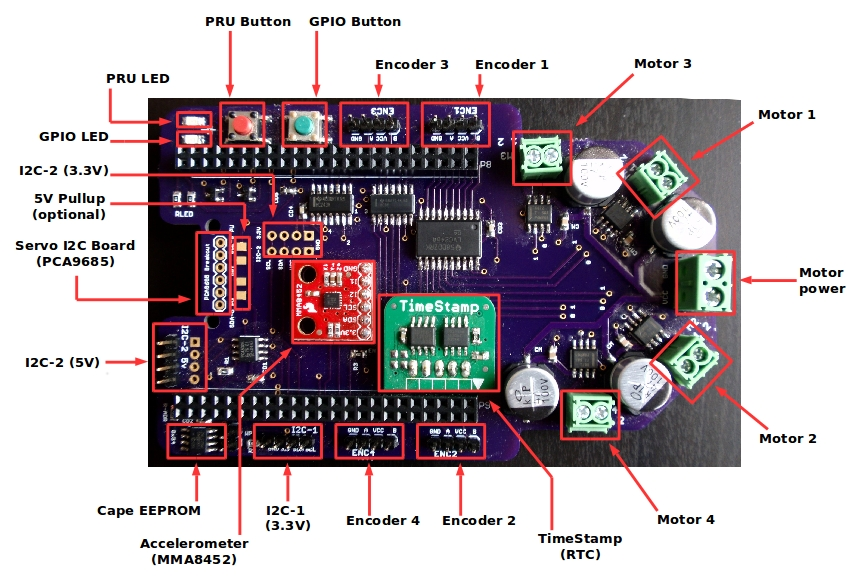
\includegraphics[scale=.4,keepaspectratio=true]{./images/BoardDiagram.jpg}
% \caption{SIUE Robot Cape}
% \label{fig:board_diagram}
%\end{figure}

%I put in the updated board diagram picture

Table from image: 

\begin{table}[htbp!]
 \centering
 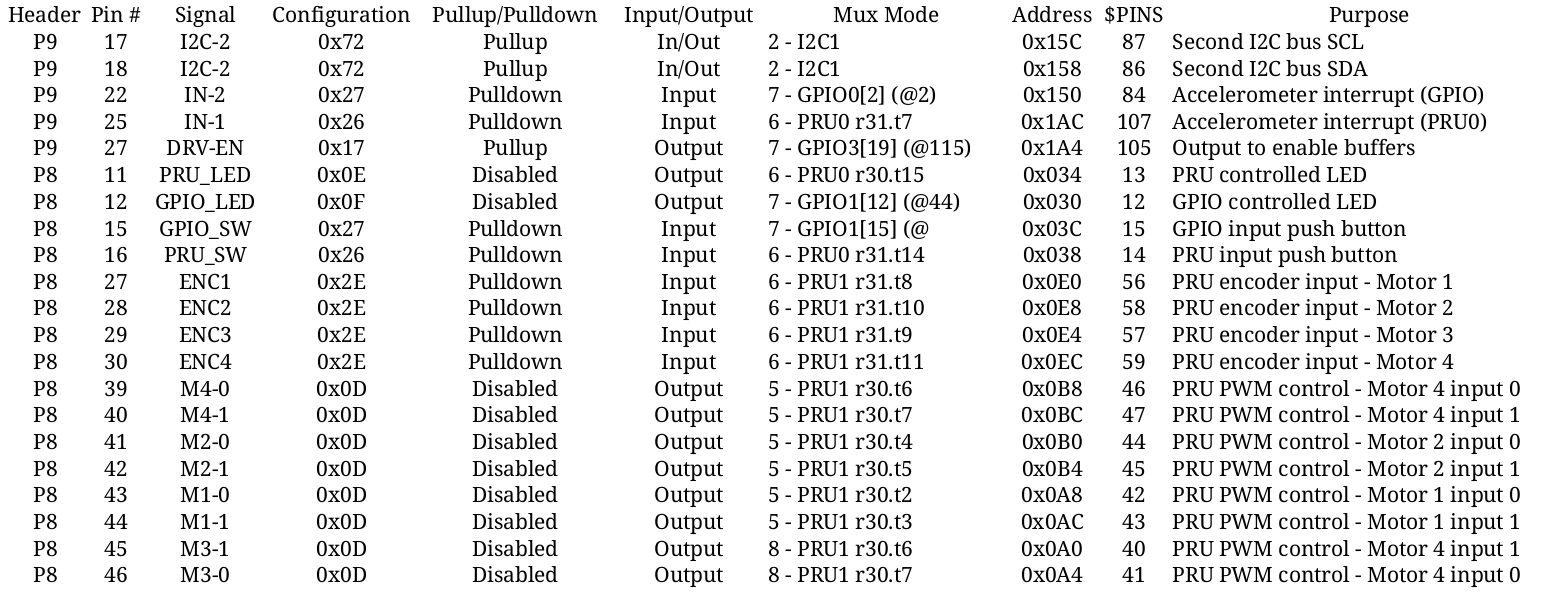
\includegraphics[scale=.3,keepaspectratio=true]{./images/Pinlist.png}
 \caption{BeagleBone Black Pins Used by SIUE Robot Cape}
 \label{tab:Pin_list}
\end{table}

Units example (mu): 47 $\mu$F

Plus/minus signs: $\pm$2g, $\pm$4g, and $\pm$8g 

Sideways figure:

\begin{sidewaysfigure}[htbp!]
 \centering
 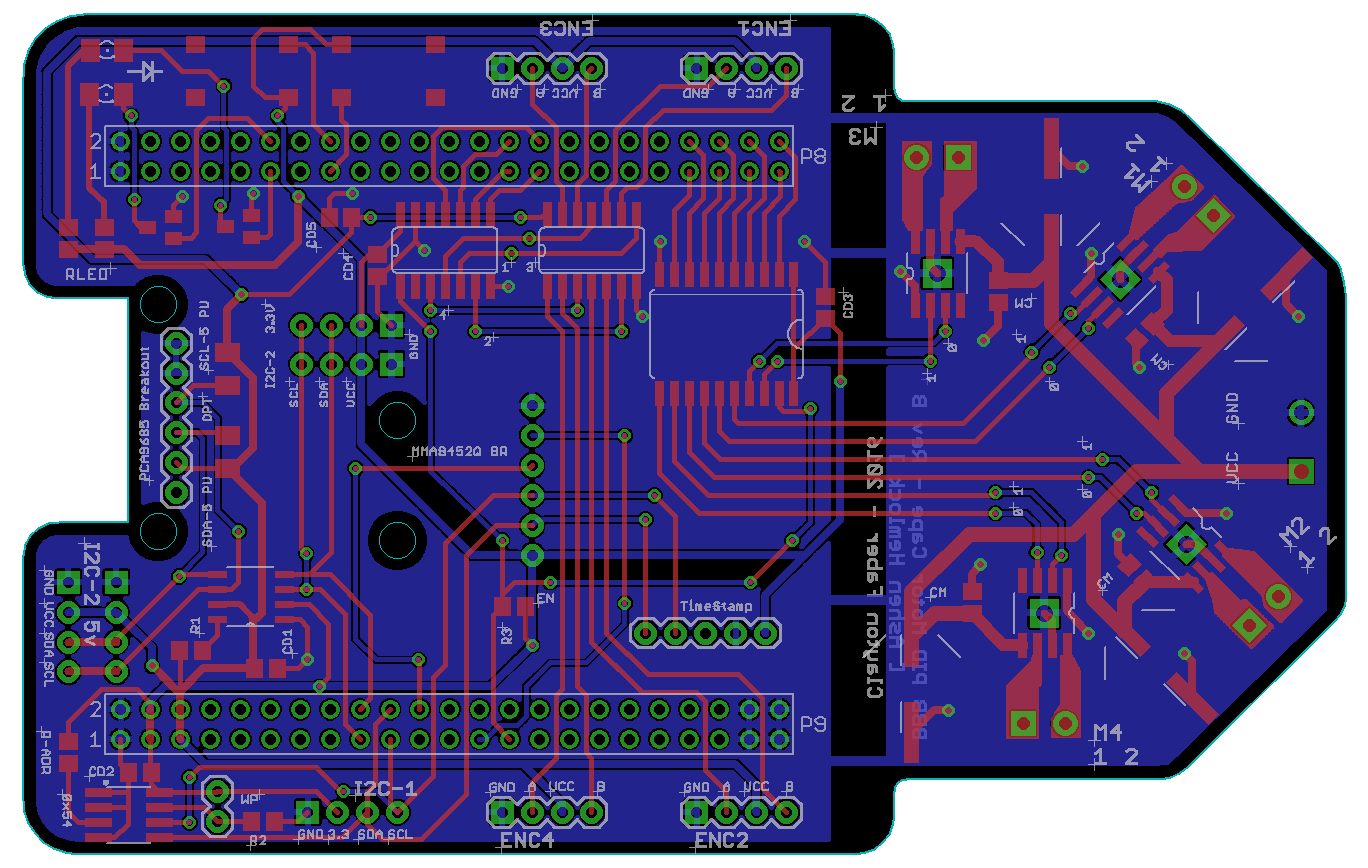
\includegraphics[scale=.5,keepaspectratio=true]{./images/layout.PNG}
 \caption{PCB Layout of SIUE Robot Cape}
 \label{fig:Layout}
\end{sidewaysfigure}


\chapter{Circuit Level Design}
Equation Array:

\begin{eqnarray}
pwm(n) &=& pwm(n-1) + \Delta(n) \\
\Delta(n) &=& \Delta_p(n) + \Delta_i(n) + \Delta_d(n) \nonumber \\
\Delta_p(n) &=& K_p \cdot e(n) \nonumber \\
\Delta_i(n) &=& K_i \cdot \left[ e(n) - e(n-1) \right] \nonumber \\
\Delta_d(n) &=& K_d \cdot \left[ e(n) - e(n-1) + 2 \cdot e(n-2) \right] \nonumber
\end{eqnarray}

Tabular table:

\begin{table}
    \begin{tabular}{ | c | p{11cm} |}
    	\hline
	Macros & Usage and Description  \\ \hline
	
	\multirow{2}{*} {get\_state} & Usage: get\_state \\& Update the status register value in pru1. b0 contains wheel control information, while b1-2 contain flag bits.
	Can be updated in shared memory from PRU0 or ARM \\ \hline

	\multirow{2}{*}{read\_clk\_cnt} & Usage: read\_clk\_cnt \\& Reads in the number of PWM cycles to run before interrupting PRU0. \\ \hline

	\multirow{2}{*}{read\_pwm\_res} & Usage: read\_pwm\_res \\ & Reads in the pwm maximum count from sharedMemory. Either 255 (8 bit), 1023 (10 bit), or 4095 (12 bit) \\ \hline

	\multirow{2}{*}{read\_pwm\_values} & Usage: read\_pwm\_values \\ & Reads in PWM high time from Shared Memory \\ \hline

	\multirow{3}{*} {pwm\_timer} & Usage:\\& pwm\_timer M\#\_ctrl, pwm\#, M\#\_1, M\#\_0, NEXT\_LINE \\ &
	This decrements the PWM register given the timer register and will stop the pwm signal if necessary. \\ \hline

	\multirow{2}{*}{pwm\_start} & Usage: pwm\_start \\ & Uses the state register to start the PWM singal using values stored in statReg.b0 \\ \hline

	

	\end{tabular}	
    \caption{PRU 1 Macros (1 of 2)}
 	\label{Tab:PRU1_Macro1}
\end{table}



escape sequence for underscore \\
check\_encoder\_edges 

Superscript: \emph{Makeblock}\textsuperscript{\textregistered}

Newpage marker:

\newpage
\begin{figure}[!t]
 \centering
 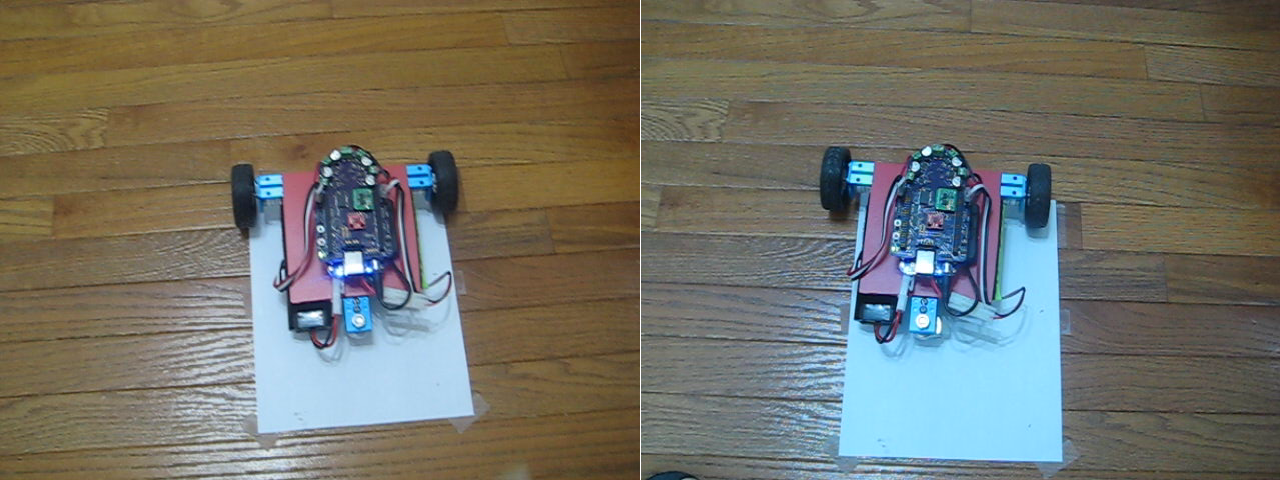
\includegraphics[scale=.35,keepaspectratio=true]{./images/robot-test1.png}
 \caption{Robot Before (left) and After (right) Run - Trial \#1}
 \label{fig:robottest1}
\end{figure}

\begin{figure}[!t]
 \centering
 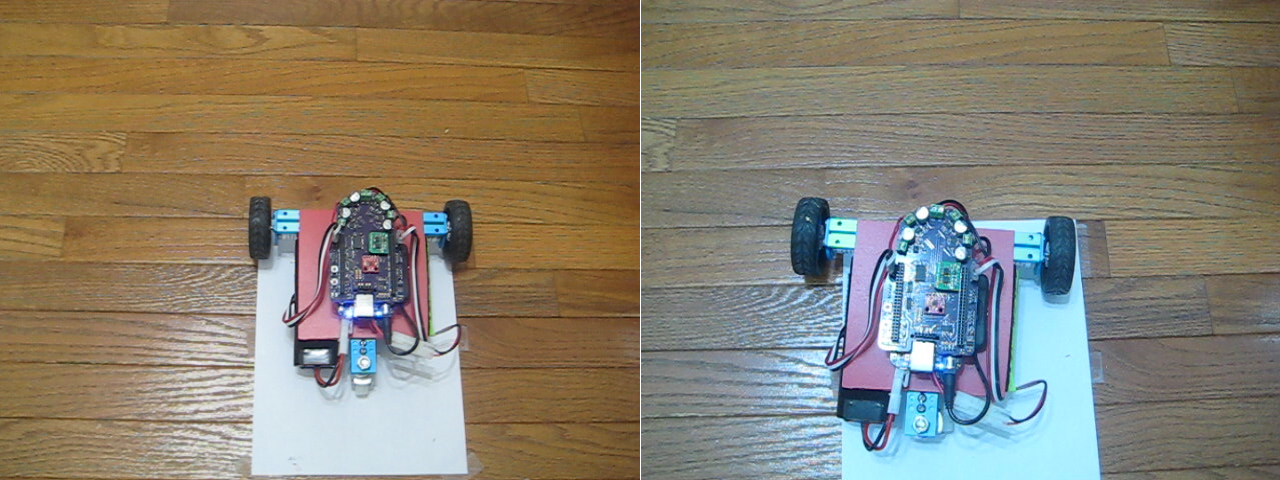
\includegraphics[scale=.35,keepaspectratio=true]{./images/robot-test2.png}
 \caption{Robot before (left) and after (right) After Run, - Trial \#2}
 \label{fig:robottest2}
\end{figure}

\chapter{Simulation}

\chapter{SUMMARY, CONCLUSIONS, AND FUTURE WORK}

\section{Summary}



\section{Conclusions}



\section{Future Work}

References and bibliography:

\references %single spacing / arabic numeral paginations, adds "REFERENCES" to table of contents

%%%% for bibtex

%If you want to use bibtex  use the following lines, where your .bib file is called 'yourbib.bib'

\bibliographystyle{apalike}
\bibliography{./cfaber_thesis}

% If you have only a single appendix, do it this way.
Appendicies: 


\multipleappendices
\lstset{
         language=C,
         basicstyle=\scriptsize\ttfamily,
         emptylines=0, 
         lineskip=1pt,
         %numbers=left,            
         numberstyle=\tiny,         
         stepnumber=2,              
         numbersep=5pt,             
         tabsize=3,                
         extendedchars=true,       
         breaklines=true,            
         commentstyle=\color{blue},
         keywordstyle=\color{red},
            frame=b,         
 %        keywordstyle=[1]\textbf,    
 %        keywordstyle=[2]\textbf,    
 %        keywordstyle=[3]\textbf,  
 %        keywordstyle=[4]\textbf,   \
         stringstyle=\scriptsize\color{green}\ttfamily, 
         showspaces=false,         
         showtabs=false,            
%         xleftmargin=17pt,
%         framexleftmargin=17pt,
%         framexrightmargin=5pt,
%         framexbottommargin=4pt,
         %backgroundcolor=\color{lightgray},
         showstringspaces=false           
 }

\chapter{Global Defines and Structures}
\lstinputlisting{./include/mem.h}

\chapter{GUI Tcl/Tk Code}
language change:

\lstset{language=[tk]tcl}
\lstinputlisting{./tcl/gui.tcl}
\end{document}
